\documentclass[a4paper,12pt,notitlepage]{mwrep}
%%\documentclass[polish,11pt,a4paper,twosides]{article}
%%%\usepackage{fullpage}

\usepackage{./mystyle}

\begin{document}

% na potrzeby strony tytułowej robimy taki nagłówek : 
\newcommand{\cfoottext}{Kraków, \today}
\renewcommand{\footrulewidth}{0.4pt}
\cfoot{\cfoottext}

\begin{titlepage}
\begin{center}
  \resizebox{\textwidth}{!}{\mbox{AKADEMIA GÓRNICZO-HUTNICZA}}\\
  \vspace{2ex}
  \resizebox{\textwidth}{!}{\mbox{Wydział Informatyki, Elektroniki i Telekomunikacji}}\\
  \vspace{4ex}
  
\includegraphics[scale=0.15]{images/agh_crop.pdf} \\
  \vspace{4ex}
  \begin{large}KATEDRA INFORMATYKI\end{large} \\
  \vspace{8ex}
  \textbf{\begin{Huge}Wielowymiarowy problem plecakowy\end{Huge}} \\
  \vspace{3ex}
  \textit{\begin{Large}Algorytm pszczeli\end{Large}} \\

  \vfill

  \begin{Large}\wersja\end{Large}\\
\end{center}
\begin{large}
  \begin{tabularx}{\textwidth}{lXc}
    \textit{Kierunek, rok studiów} &  & \textit{ } \\
    \hspace{3em}Informatyka, rok III &  &  \\
    \textit{Przedmiot} &  & \\
	\multicolumn{3}{l}{\hspace{3em}Badania Operacyjne} \\
    \textit{Prowadzący przedmiot} &  & \textit{rok akademicki:} \hfill 2012/2013\\
    \hspace{3em}dr inż. Joanna Kwiecień &  & \textit{semestr:} \hfill zimowy\\
  \end{tabularx}
\end{large}

\vspace{2ex}

\noindent
\begin{Large}
Skład zespołu:\end{Large}
\begin{large}
  \newlength{\tblwidth}
  \setlength{\tblwidth}{\textwidth}
  \addtolength{\tblwidth}{-3em}
  \begin{flushright}
    \begin{tabularx}{\tblwidth}{lXr}
      Martyna Wałaszewska &  &  \\
      Rafał Szalecki &  &  \\
      Wojciech Krzystek &  &  \\
      Grzegorz Wilaszek &  &  \\
    \end{tabularx}\end{flushright}
  \end{large}
  \thispagestyle{fancy}
\end{titlepage}



\onehalfspacing

\lhead{\scriptsize{Wałaszewska, Szalecki, Krzystek, Wilaszek}}

\lfoot{\scriptsize{Copyright \textcopyright 2012 AGH}}
\cfoot{\normalsize Strona \thepage \ z \pageref{LastPage}}
\rfoot{\scriptsize{\wersja}}
\setcounter{secnumdepth}{2}

\setcounter{tocdepth}{2}


\vfill
\begin{center}
\singlespacing
\fbox{\begin{minipage}{0.8\textwidth}
\footnotesize Niniejsze opracowanie powstało w trakcie i jako rezultat zajęć dydaktycznych z przedmiotu 
wymienionego na stronie tytułowej, prowadzonych w Akademii Górniczo-Hutniczej w Krakowie
(AGH) przez osobę (osoby) wymienioną (wymienione) po słowach "Prowadzący zajęcia"
i nie może być wykorzystywane w jakikolwiek sposób i do jakichkolwiek celów, 
w całości lub części, w szczególności publikowane w jakikolwiek sposób
i w jakiejkolwiek formie, bez uzyskania uprzedniej, pisemnej zgody tej
osoby (tych osób) lub odpowiednich władz AGH.
\vspace{2ex} \\
\textbf{Copyright \textcopyright 2012 Akademia Górniczo-Hutnicza (AGH) w Krakowie}
      \end{minipage}
}
\onehalfspacing
\end{center}

\tableofcontents

\chapter{Tematyka projektu}
\section{Opis zadania}
Zadaniem projektowym jest zaimplementowanie w dowolnie wybranej technologi aplikacji
realizującej aproksymację rozwiązania wybranego problemu NP-trudnego
za pomocą tzw. algorytmu stadnego (ang. \emph{swarm intelligence}).\\
Nasz zespół wybrał wielowymiarowy problem plecakowy, a jako algorytm:
algorytm pszczeli.
Aplikacja powinna udostępniać pewien sposób wprowadzania danych wejściowych algorytmu,
oraz powinna przedstawiać wyniki działania algorytmu w określony z prowadzącą sposób.\de
Zostały ustalone do zrealizowania 2 rodzaje prezentacji wyników działania algorymtu:
\begin{enumerate}
	\item	Wykres całkowitej wartości plecaków wziętych do plecaka
			w zależności od numeru iteracji
	\item	Widok odpowiadający na pytanie: ''Czy dany przedmiot został wzięty
			do plecaka w danej iteracji ?''
			Forma widoku dowolna.
\end{enumerate}

\section{Wielowymiarowy problem plecakowy}
\subsection{Definicja}
W ramach projektu zajmiemy się rozwiązywaniem wielowymiarowego problemu plecakowego.
Problem ten zdefiniowany jest następująco.

Dany jest zbiór $n$ przedmiotów. $j$-ty przedmiot $1 \le j \le n$
opisany jest przez swoją wartość~$p_j$ oraz ciąg wag
$(w_{1j}, w_{2j}, \dots, w_{mj})$, gdzie $m$ to liczba wymiarów.\\
Ponadto dany jest ciąg ogarniczeń plecaka $(W_1, W_2, \dots, W_m)$.\\
Zadanie polega na zmaksymalizowaniu sumy
$$ \sum_{j=1}^n p_j\chi_j$$
przy jednoczesnym zachowaniu nierówności
$$\bigforall_{1 \le i \le m}\quad\sum_{j=1}^n w_{ij}\chi_j \le W_i$$
gdzie $\chi_j \in \{0, 1\}$, wartość $\chi_j=1$
oznacza użycie $j$-tego przedmiotu.

\subsection{Wielowymiarowy problem plecakowy - Intuicja}
Nie należy mylnie utożsamiać wymiarów w problemie plecakowym z 
wymiarami przestrzeni. Intuicyjnie problem można rozumieć jako zadanie
zapakowania plecaka tak, aby sumaryczna wartość (cena)
przedmiotów była jak największa.
Przy pakowaniu należy uwzględnić $m$ \textbf{niezależnych od siebie}
ograniczeń. W rzeczywistości takimi ogarniczeniami mogą być np. waga,
objętość, zawartość nadsiarczanu potasu.

Przedmiot jest opisany przez
rozmiar w każdym z wymiarów oraz wartość (cenę). Ograniczenie plecaka
$W_i$ oznacza, że suma rozmiarów zapakowanych przedmiotów w $i$-tym
wymiarze nie może przekroczyć $W_i$.

Analizowany problem nie uwzględnia położenia przedmiotów w plecaku
ani ich geometrycznych własności. Jest to konsekwencja tego, że każdy
wymiar rozpatrujemy osobno. Dlatego nie można myśleć o rozmiarach
przedmiotu jak o rozmiarach geometrycznych.

\subsection{Złożoność}
Wielowymiarowy problem plecakowy dla liczby wymiarów $m \ge 2$ jest
problemem NP-zupełnym. Tym samym nie znamy rozwiązującego go
algorytmu o złożoności wielomianowej. Dla uzyskania rozwiązania
przybliżonego możemy stosować algorytmy aproksymacyjne, np. algorytm
pszczeli.


\chapter{Algorytm pszczeli}
\section{Opis idei algorytmu}
Algorytm pszczeli należy do grupy algorytmów rojowych, czyli algorytmów optymalizacyjnych,
których działanie bazuje na właściwościach zaobserwowanych w świecie przyrody. W przypadku
algorytmów rojowych zasada działania opiera się na regułach kooperacji w rojach owadów.
Zatem zastosowany przez nas algorytm powstał na bazie obserwacji rojów pszczelich, ich metod
komunikacji i współpracy. Algorytmy rojowe, jak i podobne do nich metody optymalizacyjne,
nie budują jednego i konkretnego rozwiązania, ale bazują na zbiorze rozwiązań, które mogą być
przetwarzane równolegle, także wieloprocesowo, wielowątkowo czy też w architekturze rozproszonej.
Często są jedynym sposobem rozwiązania problemów, które w klasyczym podejściu mają złożoność obliczeniową
przekraczającą możliwości współczesnych komputerów.

%\begin{figure}[H] % H - Places the float at precisely the location in the LaTeX code.
%\centering
%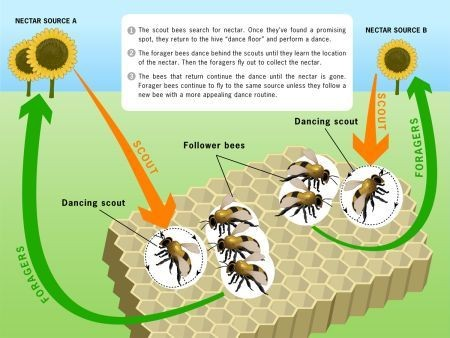
\includegraphics[width=1.05\textwidth]{pszczoly.jpeg}
%\caption{Schemat działania pszczół\ldots czy jakoś tak}
%\label{fig:Pszczoly}
%\end{figure}

\subsection{Główne obserwacje}
Podstawowe założenia algorytmu opierają się na pewnych zasadach zaobserwowanych we współpracy pszczelej kolonii.
Pszczoły opuszczeją swoje siedlisko, ul, na spore odległości w poszukiwaniu pyłku kwiatów.
Organizacja ich wspólpracy wygląda następująco. Wysyłani są pszczeli zwiadowcy, którzy losowo przemierzają pobliskie tereny,
zbierając informacje o zasobach. Ważna jest odległość od ula, ilość zasobów oraz oczywiście ich lokalizacja. Posiadając takie
informacje, zwiadowca wraca do ula i wykonuje specjalny taniec, który ma poinformować inne pszczoły o wnikach zwiadu.
Kierunek tańca pokazuje lokalizację znalezionych zasobów. Czas trwania tańca oznacza odległość znalezionych zasobów
od ula, a intensywność ruchów podczas pokazu świadczy o ilości odnalezionych pyłków kwiatowych. W zależności od zaprezentowanego
tańca, odpowiednia część roju udaje się we wskazane miejsce, gdzie zbiera pyłek z kwiatów i wraca do ula. Po powrocie przekazuje
reszcie roju aktualne informacje o zasobie, co pozwala na kolejne podejmowania decyzji o oksploatacji zasobów i wysyłaniu w dane
miejsce kolejnych pszczół.

\subsection{Odzwierciedlenie w algorytmie}
Opisane powyżej mechanizmy przekładają się na strategię algorytmu w różnych jego etapach.
Oto podstawowe skojarzania pszczelich zwyczajów w odniesieniu do zadań, które ma wykonać algorytm:\\

\begin{tabular}{|l|l|}
\hline
Element pszczelej kolonii & Odzwierciedlenie w algorytmie \\
\hline
Teren wokół ula & Zbiór możliwych rozwiązań \\
Lokalizacja nektaru & Pewne rozwiązanie \\
Ilość nektaru & Wartość funkcji celu \\
Pszczoły-zwiadowcy & Losowo inicjowane początkowe rozwiązania \\
Populacja pszczół & Przeszukiwanie sąsiedztwa danego rozwiązania \\
Zużycie się zasobów & Porzucanie lokalnych maksimów po \\
& przeszukaniu pewnej ilości sąsiedztw \\
\hline
\end{tabular}\\

Można krótko przedstawić ogólny zarys i ideę rozwiązywania problemów algorytmem pszczelim:
\begin{enumerate}
	\fe	Utworzenie $n$ początkowych populacji i wyznaczenie dla nich wartości funkcji celu.
	\fe	Wybór $m$ przeszukiwanych sąsiedztw i określenie ich wielkości oraz liczności rozwiązań dla nich.
	\fe	Według zadanej wielkości i liczności utworzenie rozwiązań dla każdego z m sąsiedztw oraz wyznaczenie dla nich wartości funkcji celu.
	\fe	Utworzenie nowej populacji $n$ rozwiązań (przez wybór najlepszych rozwiązań dla każdego z $n$ sąsiedztw oraz uzupełnienie brakujących $n-m$ rozwiązań).
	\fe	Jeśli spełniony jest warunek stopu, to kończymy. W przeciwnym wypadku: POWRÓT DO 2.
\end{enumerate}

\chapter{Implementacja rozwiązująca wielowymiarowy problem plecakowy}
\section{Dane}
Danymi wejściowymi dla algorytmu są:
\begin{itemize}
\item Instancja problemu plecakowego -- oznaczenia jak w definicji
\item Parametry sterujące algorytmem
\begin{itemize}
\item $nBee$ ilość rozpatrywanych rozwiązań (dostępnych pszczół)
\item $nSite$ ilość najlepszych rozwiązań wybranych do przeszukiwania sąsiedztwa
\item $ngh$ rozmiar przeszukiwanego sąsiedztwa
\item $nep$ ilość pszczół przeznaczona do przeszukiwania sąsiedztw
\item $maxIterations$ liczba iteracji
\end{itemize}
\end{itemize}
%\section{Algorytm}
%Algorytm przedstawiony przy pomocy pseudokodu:
%\begin{enumerate}
%	\fe	
%\end{enumerate}

\chapter{Opis aplikacji}
\section{Uruchamianie}
Aplikacja została zrealizowana w technologi Java, dlatego do jej uruchomienia będzie
potrzebne środowisko JRE\footnote{Bądź JDK} w wersji 1.7 lub nowszej.
Znajdując się w katalogu, w którym został umieszczony plik \texttt{knabees-1.0-jar-with-dependencies.jar}
należy wydać polecenie:
\begin{verbatim}
java -jar knabees-1.0-jar-with-dependencies.jar
\end{verbatim}
Użytkownikowi powinno ukazać się główne okno aplikacji z aktywną zakładką ustalania parametrów
algorytmu.

\section{Działanie aplikacji}
Startowe okno aplikacji podzielono na dwie części -- zakładki:
\begin{enumerate}
	\item	Zakładkę ustawiania parametrów algorytmu
	\item	Zakładkę wprowadzania parametrów plecaka i przedmiotów
\end{enumerate}
Pomiędzy zakładkami możemy się swobodnie poruszać.
\begin{figure}[H]
\centering
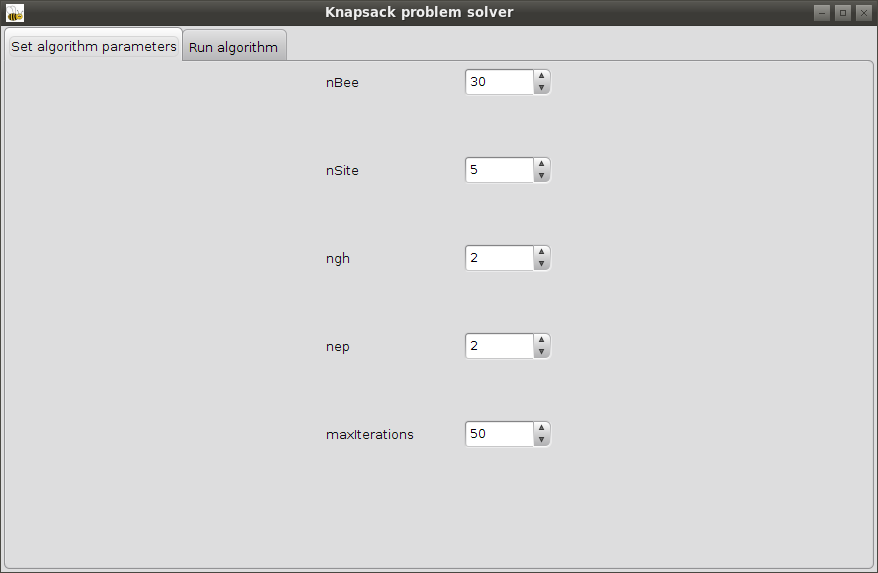
\includegraphics[width=1.0\textwidth]{params.png}
\caption{Aplikacja zaraz po uruchomieniu --- zakładka ustawiania parametrów algorytmu}
\label{fig:params}
\end{figure}

\subsection{Ładowanie danych wejściowych}
W drugiej zakładce mamy dostępne dwie metody ładowania parametrów plecaka oraz przedmiotów:
\begin{enumerate}
	\item	\textsc{Ładowanie z pliku tekstowego}.\\
			Format danych powinien być zgodny z tym opisanym w \ref{format}.
			Należy przycisnąć przycisk ''Load items\&knapsack'', pojawi się nowe okno, w którym możemy wybrać plik z danymi.
			Jeżeli format pliku jest poprawny w odpowiednie pole tekstowe zostaną załadowane wymiary plecaka,
			oraz zostanie wypełniona lista przedmiotów.
			O powodzeniu parsowania pliku informować będzie pole statusu po prawej stronie przycisku ładowania pliku.
			(Patrz: Rysunek \ref{fig:load})\\
			\textbf{Uwaga:} Ponowne załadowanie danych z pliku spowoduje \textbf{nadpisanie} plecaka nowym plecakiem,
			oraz \textbf{dodanie} nowych przedmiotów do listy, a nie usunięcie starych.
			\begin{figure}[H]
			\centering
			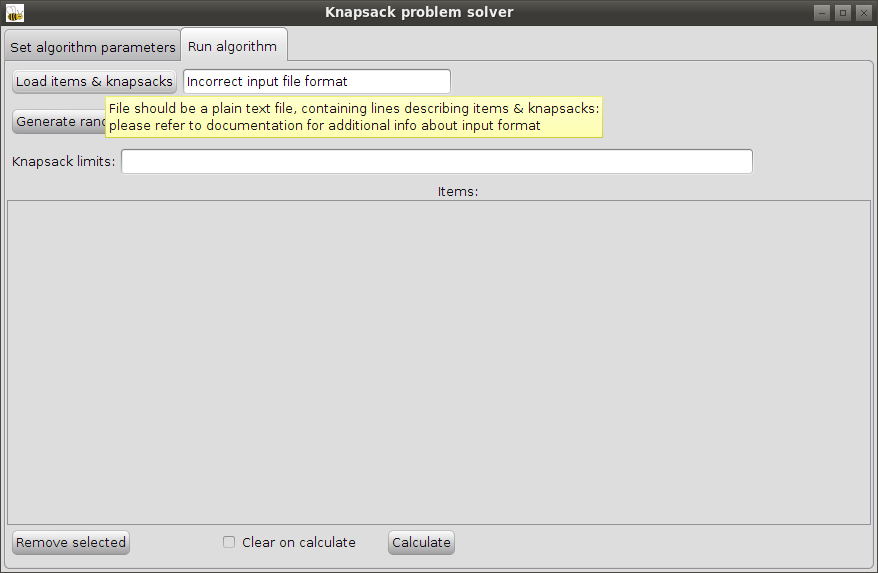
\includegraphics[width=0.8\textwidth]{file_tooltip.png}
			\caption{Ładowanie danych z pliku}
			\label{fig:load}
			\end{figure}
	\item	\textsc{Generowanie losowych danych}
			Pojawi się dodatkowe okno, w którym mozemy ustawić parametry danych losowych.
			Dostępne parametry generowania losowego przedstawia rysunek \ref{fig:generate}.\\
			\textbf{Uwaga:} Ponowne wygenerowanie danych losowych spowoduje \textbf{nadpisanie}
			zarówno plecaka jak i przedmiotów nowymi danymi.
			\begin{figure}[H]
			\centering
			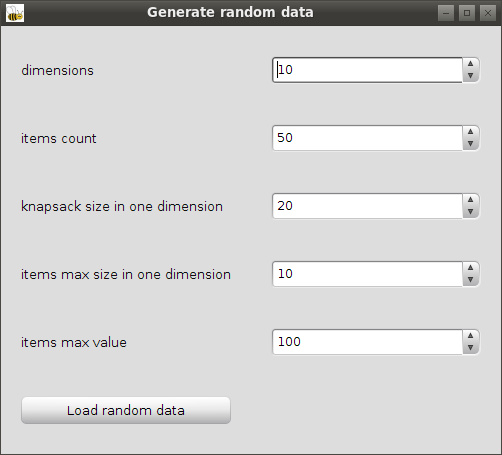
\includegraphics[width=0.8\textwidth]{generate.png}
			\caption{Okno generowania losowych danych}
			\label{fig:generate}
			\end{figure}
\end{enumerate}
Po załadowaniu danych będą one widoczne w tej samej zakładce (Rysunek \ref{fig:ki}).
Przed uruchomieniem algorytmu mamy możliwość usunięcia wybranych przedmiotów z listy.
Obliczenia uruchamiamy wciskając przycisk ''Calculate''.
Zaznaczenie flagi ''Clear on calculate'' spowoduje skasowanie danych plecaka i przedmiotów.\\
Jeśli chcemy testować działanie algorytmu na tych samych danych wielokrotnie,
należy flagę odznaczyć (domyślnie jest odznaczona).

\begin{figure}[H]
\centering
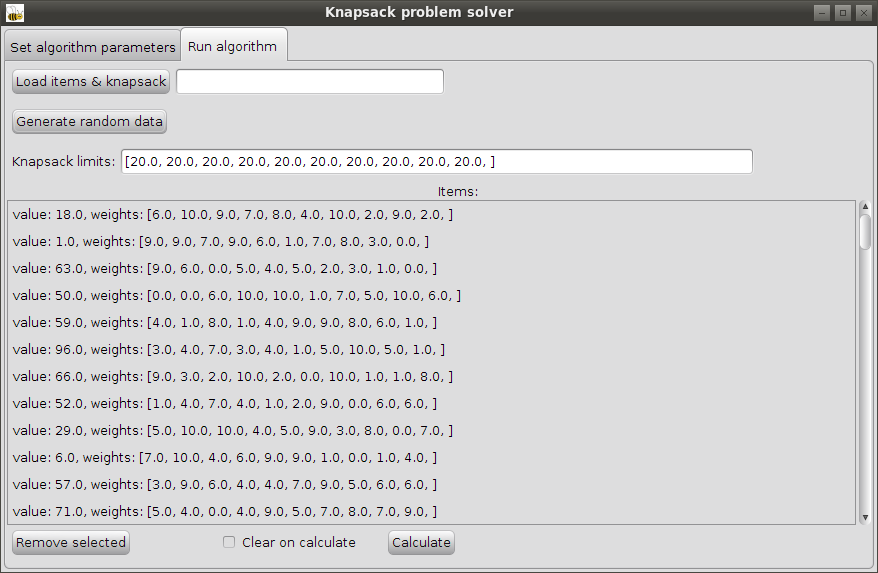
\includegraphics[width=1.0\textwidth]{k&i.png}
\caption{Załadowane dane}
\label{fig:ki}
\end{figure}

\subsection{Prezentacja wyników obliczeń}
Po uruchomieniu algorytmu pojawią się dwa okna:
\begin{enumerate}
	\item	Wykres zmian całkowitej wartości przedmiotów wziętych do plecaka
			w zależności od numeru iteracji.\\
			\begin{figure}[H]
			\centering
			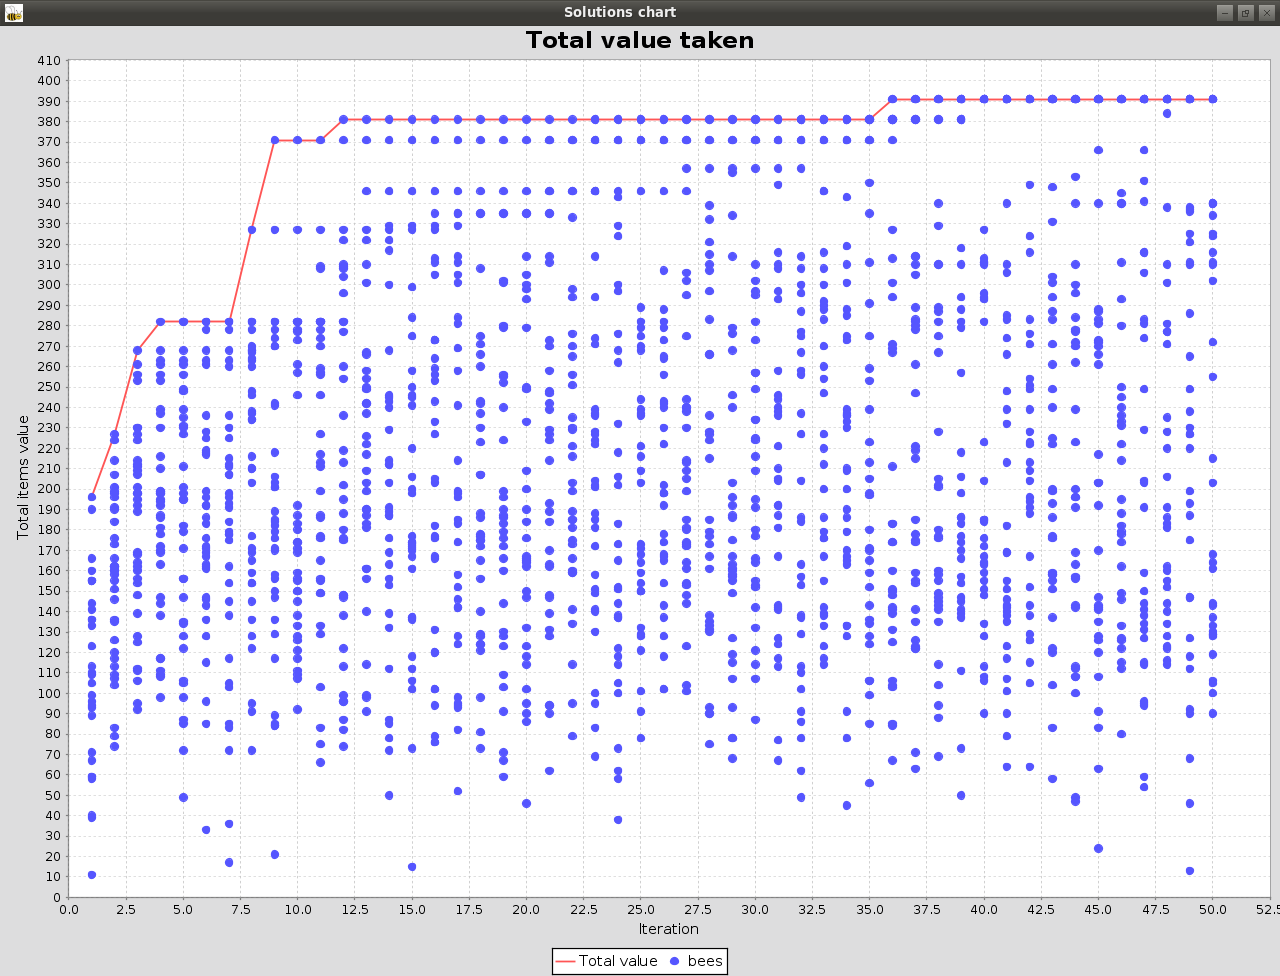
\includegraphics[width=1.0\textwidth]{chart.png}
			\caption{Wykres}
			\label{fig:chart}
			\end{figure}
			Dodatkowo wykres prezentuje intrygujące skupiska niebieskich kropek.\\
			Przyczyny ich powstawania do dziś pozostają niewyjaśnioną przez
			naukowców tajemnicą. // FIXME, TODO
	\item	Okno statusu (wybrany / niewybrany) przedmiotów w danej iteracji.\\
			\begin{figure}[H]
			\centering
			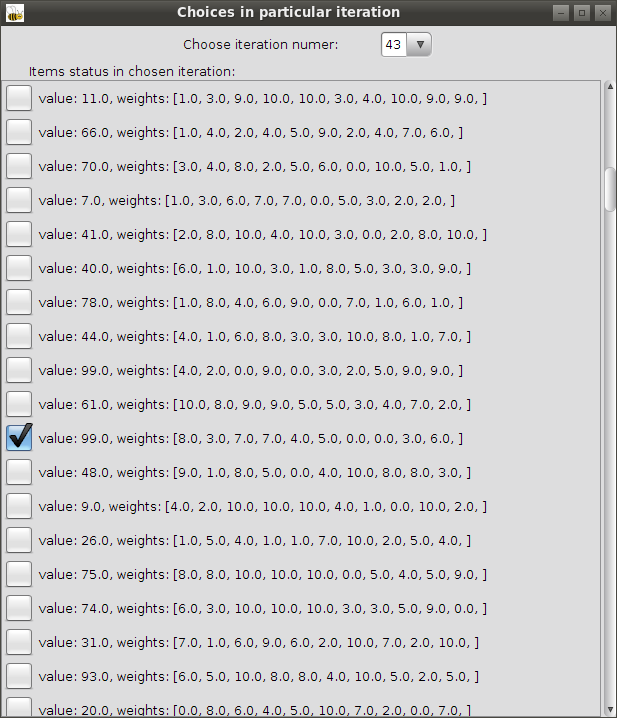
\includegraphics[width=0.8\textwidth]{chosen_items.png}
			\caption{Okno statusu przedmiotów}
			\label{fig:chosen_items}
			\end{figure}
			Używając listy rozwijanej na górze możemy wybrać numer iteracji,
			lista automatycznie zostanie odświeżona danymi z wybranej iteracji.
			Pusty, szary kwadracik oznacza przedmiot niewybrany, kwadracik z niebiesko-czarnym
			zaznaczeniem --- przedmiot wybrany.
\end{enumerate}
Informacje przezentowane w oknach są automatycznie odświeżane po zakończeniu iteracji
algorytmu. Na ogół zakończenie całego algorytmu (tj. wybranej liczby iteracji) następuje
stosunkowo szybko i nie mamy możliwości podglądu "na żywo".\\
\textbf{Uwaga:} Zamknięcie któregokolwiek z okien spowoduje zakończenie działania aplikacji.


\subsection{Format pliku z danymi wejściowymi} \label{format}
Plik z danymi wejściowymi problemu plecakowego powinien być następującej postaci. W pierwszej
linii wejścia znajdują się dwie liczby naturalne $m$, $n$ oznaczające kolejno liczbę wymiarów
oraz liczbę dostępnych przedmiotów. W drugiej linii wejścia znajduje się $m$~liczb rzeczywistych oddzielonych
spacjami oznaczających kolejne ograniczenia plecaka. Następne $n$ linii opisuje kolejne przedmioty.
Pojedyncza linia opisująca $j$-ty~przedmiot składa się z $m+1$~liczb rzeczywistych oddzielonych spacjami.
Pierwsza z nich to $p_j$~--~wartość (cena)
przedmiotu. Kolejne $m$ liczb oznacza kolejne rozmiary przedmiotu $w_{ij}$  ($1 \le i \le m$).


\chapter{Podsumowanie}
\section{Użyte technologie}
Aplikacja została wykonana w technologii Java 1.7
jako aplikacja stacjonarna,
dodatkowo użyto technologie pokrewne wymienione poniżej.
\begin{itemize}
	\item	\textbf{GUI}\quad Do wykonania interfejsu graficznego posłużyła biblioteka standardowa Swing
	\item	\textbf{Wykresy}\quad Do tworzenia wykresów użyto biblioteki JFreeChart w wersji 1.0.13
	\item	\textbf{Budowa}\quad Cały proces budowania i kontroli zależności był nadzorowany przez narzędzie
					Maven3
	\item	\textbf{Logowanie}\quad biblioteka Log4j 1.2.17
\end{itemize}

\section{Użyte narzędzia}
\begin{itemize}
	\item	\textbf{Dokumentacja}\quad \LaTeX
	\item	\textbf{Synchronizacja}\quad (Zarówno dokumentacja jak i kod aplikacji) : system kontroli wersji git
			z repozytowium w serwisie bitbucket
	\item	\textbf{IDE\quad} Eclipse Juno 4.2 J2EE z rozszerzeniami, m. in. m2eclipse, EGit
	\item	\textbf{System operacyjny}\quad Całość prac przeprowadzono na systemach Linux
\end{itemize}

\section{Podział pracy}
\begin{description}
	\item[Algorytm] Martyna Wałaszewska, Rafał Szalecki
	\item[Aplikacja] Grzegorz Wilaszek (wykresy), Wojciech Krzystek (aplikacja, setup)
	\item[Dokumentacja] wszyscy członkowie zespołu
\end{description}


\addtocounter{page}{-1}

\appendix
\chapter*{Zawartość płyty CD}
\begin{description}
	\item[plik main.pdf]	 --- plik z tą dokumentacją (dodatkowo dokumentacja jest oddawana w formie drukowanej)
	\item[folder knabees]	 --- folder z kompletnym kodem źródłowym aplikacji
	\item[plik knabees-1.0-jar-with-dependencies.jar]	 --- plik jar zbudowanej aplikacji Javowej
	\item[pokaz.avi]	 --- krótki filmik demonstrujący działanie aplikacji
\end{description}

\begin{thebibliography}{9}

\bibitem{enwiki}
	\href{http://en.wikipedia.org/wiki/List_of_knapsack_problems}{http://en.wikipedia.org/wiki/List\_of\_knapsack\_problems}
\bibitem{swing}
	\href{http://docs.oracle.com/javase/tutorial/uiswing/components/index.html}{Java tutorials, Lesson: Using Swing Components}
\bibitem{mvnex}
	\href{http://www.sonatype.com/Support/Books/Maven-By-Example}{Sonatype, Maven By Example}
\bibitem{mvntcr}
	\href{http://www.sonatype.com/Support/Books/Maven-The-Complete-Reference}{Sonatype, Maven: The Complete Reference}
\bibitem{progit}
	\href{http://git-scm.com/book/}{Scott Chacon, Pro Git}
\bibitem{java2s}
	\href{http://www.java2s.com/Code/Java/Chart/CatalogChart.htm}{Java2S - Programming tutorials and source code examples: Charting}
\bibitem{stack}
	\href{http://stackoverflow.com/}{Stackoverflow}

\end{thebibliography}


\listoffigures


\label{LastPage}\phantom{\phantomsection{LastPage}}
\end{document}
